\documentclass[twoside]{book}

% Packages required by doxygen
\usepackage{fixltx2e}
\usepackage{calc}
\usepackage{doxygen}
\usepackage[export]{adjustbox} % also loads graphicx
\usepackage{graphicx}
\usepackage[utf8]{inputenc}
\usepackage{makeidx}
\usepackage{multicol}
\usepackage{multirow}
\PassOptionsToPackage{warn}{textcomp}
\usepackage{textcomp}
\usepackage[nointegrals]{wasysym}
\usepackage[table]{xcolor}

% Font selection
\usepackage[T1]{fontenc}
\usepackage[scaled=.90]{helvet}
\usepackage{courier}
\usepackage{amssymb}
\usepackage{sectsty}
\renewcommand{\familydefault}{\sfdefault}
\allsectionsfont{%
  \fontseries{bc}\selectfont%
  \color{darkgray}%
}
\renewcommand{\DoxyLabelFont}{%
  \fontseries{bc}\selectfont%
  \color{darkgray}%
}
\newcommand{\+}{\discretionary{\mbox{\scriptsize$\hookleftarrow$}}{}{}}

% Page & text layout
\usepackage{geometry}
\geometry{%
  a4paper,%
  top=2.5cm,%
  bottom=2.5cm,%
  left=2.5cm,%
  right=2.5cm%
}
\tolerance=750
\hfuzz=15pt
\hbadness=750
\setlength{\emergencystretch}{15pt}
\setlength{\parindent}{0cm}
\setlength{\parskip}{3ex plus 2ex minus 2ex}
\makeatletter
\renewcommand{\paragraph}{%
  \@startsection{paragraph}{4}{0ex}{-1.0ex}{1.0ex}{%
    \normalfont\normalsize\bfseries\SS@parafont%
  }%
}
\renewcommand{\subparagraph}{%
  \@startsection{subparagraph}{5}{0ex}{-1.0ex}{1.0ex}{%
    \normalfont\normalsize\bfseries\SS@subparafont%
  }%
}
\makeatother

% Headers & footers
\usepackage{fancyhdr}
\pagestyle{fancyplain}
\fancyhead[LE]{\fancyplain{}{\bfseries\thepage}}
\fancyhead[CE]{\fancyplain{}{}}
\fancyhead[RE]{\fancyplain{}{\bfseries\leftmark}}
\fancyhead[LO]{\fancyplain{}{\bfseries\rightmark}}
\fancyhead[CO]{\fancyplain{}{}}
\fancyhead[RO]{\fancyplain{}{\bfseries\thepage}}
\fancyfoot[LE]{\fancyplain{}{}}
\fancyfoot[CE]{\fancyplain{}{}}
\fancyfoot[RE]{\fancyplain{}{\bfseries\scriptsize Generated by Doxygen }}
\fancyfoot[LO]{\fancyplain{}{\bfseries\scriptsize Generated by Doxygen }}
\fancyfoot[CO]{\fancyplain{}{}}
\fancyfoot[RO]{\fancyplain{}{}}
\renewcommand{\footrulewidth}{0.4pt}
\renewcommand{\chaptermark}[1]{%
  \markboth{#1}{}%
}
\renewcommand{\sectionmark}[1]{%
  \markright{\thesection\ #1}%
}

% Indices & bibliography
\usepackage{natbib}
\usepackage[titles]{tocloft}
\setcounter{tocdepth}{3}
\setcounter{secnumdepth}{5}
\makeindex

% Hyperlinks (required, but should be loaded last)
\usepackage{ifpdf}
\ifpdf
  \usepackage[pdftex,pagebackref=true]{hyperref}
\else
  \usepackage[ps2pdf,pagebackref=true]{hyperref}
\fi
\hypersetup{%
  colorlinks=true,%
  linkcolor=blue,%
  citecolor=blue,%
  unicode%
}

% Custom commands
\newcommand{\clearemptydoublepage}{%
  \newpage{\pagestyle{empty}\cleardoublepage}%
}

\usepackage{caption}
\captionsetup{labelsep=space,justification=centering,font={bf},singlelinecheck=off,skip=4pt,position=top}

%===== C O N T E N T S =====

\begin{document}

% Titlepage & ToC
\hypersetup{pageanchor=false,
             bookmarksnumbered=true,
             pdfencoding=unicode
            }
\pagenumbering{alph}
\begin{titlepage}
\vspace*{7cm}
\begin{center}%
{\Large Te\+Xlib }\\
\vspace*{1cm}
{\large Generated by Doxygen 1.8.13}\\
\end{center}
\end{titlepage}
\clearemptydoublepage
\pagenumbering{roman}
\tableofcontents
\clearemptydoublepage
\pagenumbering{arabic}
\hypersetup{pageanchor=true}

%--- Begin generated contents ---
\chapter{Hierarchical Index}
\section{Class Hierarchy}
This inheritance list is sorted roughly, but not completely, alphabetically\+:\begin{DoxyCompactList}
\item exception\begin{DoxyCompactList}
\item \contentsline{section}{TeX\+:\+:Te\+X\+Exception}{\pageref{class_te_x_1_1_te_x_exception}}{}
\end{DoxyCompactList}
\item \contentsline{section}{TeX}{\pageref{class_te_x}}{}
\end{DoxyCompactList}

\chapter{Class Index}
\section{Class List}
Here are the classes, structs, unions and interfaces with brief descriptions\+:\begin{DoxyCompactList}
\item\contentsline{section}{\hyperlink{class_te_x}{TeX} }{\pageref{class_te_x}}{}
\item\contentsline{section}{\hyperlink{class_te_x_1_1_te_x_exception}{Te\+X\+::\+Te\+X\+Exception} }{\pageref{class_te_x_1_1_te_x_exception}}{}
\end{DoxyCompactList}

\chapter{Class Documentation}
\hypertarget{class_te_x}{}\section{TeX Class Reference}
\label{class_te_x}\index{TeX@{TeX}}


{\ttfamily \#include $<$texlib.\+h$>$}

\subsection*{Classes}
\begin{DoxyCompactItemize}
\item 
class \hyperlink{class_te_x_1_1_te_x_exception}{Te\+X\+Exception}
\end{DoxyCompactItemize}
\subsection*{Public Member Functions}
\begin{DoxyCompactItemize}
\item 
\hyperlink{class_te_x_aab21a09cfa857de0126d81b9f5743417}{TeX} (bool show\+\_\+shell=false)
\item 
\hyperlink{class_te_x_a2f70e397b6e5136c7ba421fe82bd5f4d}{TeX} (std\+::string filename, bool show\+\_\+shell=false)
\item 
\hyperlink{class_te_x_ade9e129defdfd30770f256aa178684a3}{$\sim$\+TeX} ()
\item 
{\footnotesize template$<$typename string\+\_\+convertable $>$ }\\std\+::ostream \& \hyperlink{class_te_x_ad82a6fa685379180ba717d341295b89c}{operator$<$$<$} (const string\+\_\+convertable to\+\_\+be\+\_\+written)
\item 
void \hyperlink{class_te_x_a0480cb8479c2c5c3704d573c2b945d92}{to\+\_\+pdf} ()
\item 
\mbox{\Hypertarget{class_te_x_a3943ff1c49684fddbbecfde268bdd89e}\label{class_te_x_a3943ff1c49684fddbbecfde268bdd89e}} 
void {\bfseries to\+\_\+dvi} ()
\item 
std\+::string \hyperlink{class_te_x_ad1602a89751db15a14ce7be506ed94b9}{to} (std\+::string ext, std\+::string middle\+\_\+ext=\char`\"{}pdf\char`\"{})
\item 
void \hyperlink{class_te_x_acc84be2a6474f7a354c0dbc5b312637f}{set\+\_\+image\+\_\+density} (const int density)
\item 
\mbox{\Hypertarget{class_te_x_a9406e9e82feeddbcd9c6cb2e8cef341c}\label{class_te_x_a9406e9e82feeddbcd9c6cb2e8cef341c}} 
int {\bfseries get\+\_\+image\+\_\+density} () const
\item 
bool \hyperlink{class_te_x_a742040deabcc5e71e314a3e3cf7deaa6}{open} ()
\item 
bool \hyperlink{class_te_x_abcc58201c7ea70c660e22aa633be2c3a}{open\+\_\+rewritemode} ()
\item 
void \hyperlink{class_te_x_ac3807f2a31df4bc40cf679e4f60b87c7}{open} (std\+::string filename)
\item 
void \hyperlink{class_te_x_a6b702106c0b4391ba8bd28aa50298074}{close} ()
\item 
bool \hyperlink{class_te_x_a7dd90c338d4225d8ed2950323d366520}{exists} ()
\item 
{\footnotesize template$<$typename T  = std\+::string$>$ }\\void \hyperlink{class_te_x_a72321520da5083a03a5e80df58236fca}{do\+\_\+not\+\_\+cancel} (T extenstion)
\item 
{\footnotesize template$<$typename T  = std\+::string, typename... Types$>$ }\\void \hyperlink{class_te_x_acf8a041cbb39d209b72c66ebec52be99}{do\+\_\+not\+\_\+cancel} (T extenstion, Types... others)
\item 
void \hyperlink{class_te_x_a788c3b484fdcc4797915044b9c6e67aa}{rmfiles} ()
\item 
std\+::string \hyperlink{class_te_x_aacfd237cb2f7ea19afe01895fc1987dc}{get\+\_\+name} () const
\item 
path \hyperlink{class_te_x_a8252aa7134ebc330a8b3da6462f13aeb}{get\+\_\+path} () const
\item 
std\+::string \hyperlink{class_te_x_a18399db9f0d97b7c06e7fa72d1a146c4}{get\+\_\+fullpath\+\_\+ext} (std\+::string extension) const
\end{DoxyCompactItemize}


\subsection{Detailed Description}
This class is a \hyperlink{class_te_x}{TeX} quick-\/compiler\+: it basically converts small portions of tex code to pdf or png. It is not designed to handle a proper tex file (reason for which it the methods to write and compile are implemented in the same class), even though, with little modification, it can be used as such.

\{T\+EX\} 

\subsection{Constructor \& Destructor Documentation}
\mbox{\Hypertarget{class_te_x_aab21a09cfa857de0126d81b9f5743417}\label{class_te_x_aab21a09cfa857de0126d81b9f5743417}} 
\index{TeX@{TeX}!TeX@{TeX}}
\index{TeX@{TeX}!TeX@{TeX}}
\subsubsection{\texorpdfstring{Te\+X()}{TeX()}\hspace{0.1cm}{\footnotesize\ttfamily [1/2]}}
{\footnotesize\ttfamily Te\+X\+::\+TeX (\begin{DoxyParamCaption}\item[{bool}]{show\+\_\+shell = {\ttfamily false} }\end{DoxyParamCaption})}

Default creator 
\begin{DoxyParams}{Parameters}
{\em show\+\_\+shell} & if true shows shell information when executing shell commands (La\+TeX compilation) \\
\hline
\end{DoxyParams}
\mbox{\Hypertarget{class_te_x_a2f70e397b6e5136c7ba421fe82bd5f4d}\label{class_te_x_a2f70e397b6e5136c7ba421fe82bd5f4d}} 
\index{TeX@{TeX}!TeX@{TeX}}
\index{TeX@{TeX}!TeX@{TeX}}
\subsubsection{\texorpdfstring{Te\+X()}{TeX()}\hspace{0.1cm}{\footnotesize\ttfamily [2/2]}}
{\footnotesize\ttfamily Te\+X\+::\+TeX (\begin{DoxyParamCaption}\item[{std\+::string}]{filename,  }\item[{bool}]{show\+\_\+shell = {\ttfamily false} }\end{DoxyParamCaption})}


\begin{DoxyParams}{Parameters}
{\em filename} & \hyperlink{class_te_x}{TeX} file to be opened \\
\hline
\end{DoxyParams}
\mbox{\Hypertarget{class_te_x_ade9e129defdfd30770f256aa178684a3}\label{class_te_x_ade9e129defdfd30770f256aa178684a3}} 
\index{TeX@{TeX}!````~TeX@{$\sim$\+TeX}}
\index{````~TeX@{$\sim$\+TeX}!TeX@{TeX}}
\subsubsection{\texorpdfstring{$\sim$\+Te\+X()}{~TeX()}}
{\footnotesize\ttfamily Te\+X\+::$\sim$\+TeX (\begin{DoxyParamCaption}{ }\end{DoxyParamCaption})}

Destructor Removes the last file created and the compilation temporary file. If certains extentions are not to be removed they should be passed to the function do\+\_\+not\+\_\+cancel(ext). 

\subsection{Member Function Documentation}
\mbox{\Hypertarget{class_te_x_a6b702106c0b4391ba8bd28aa50298074}\label{class_te_x_a6b702106c0b4391ba8bd28aa50298074}} 
\index{TeX@{TeX}!close@{close}}
\index{close@{close}!TeX@{TeX}}
\subsubsection{\texorpdfstring{close()}{close()}}
{\footnotesize\ttfamily void Te\+X\+::close (\begin{DoxyParamCaption}{ }\end{DoxyParamCaption})\hspace{0.3cm}{\ttfamily [inline]}}

Closes the current opened file if any. \mbox{\Hypertarget{class_te_x_a72321520da5083a03a5e80df58236fca}\label{class_te_x_a72321520da5083a03a5e80df58236fca}} 
\index{TeX@{TeX}!do\+\_\+not\+\_\+cancel@{do\+\_\+not\+\_\+cancel}}
\index{do\+\_\+not\+\_\+cancel@{do\+\_\+not\+\_\+cancel}!TeX@{TeX}}
\subsubsection{\texorpdfstring{do\+\_\+not\+\_\+cancel()}{do\_not\_cancel()}\hspace{0.1cm}{\footnotesize\ttfamily [1/2]}}
{\footnotesize\ttfamily template$<$typename T  = std\+::string$>$ \\
void Te\+X\+::do\+\_\+not\+\_\+cancel (\begin{DoxyParamCaption}\item[{T}]{extenstion }\end{DoxyParamCaption})\hspace{0.3cm}{\ttfamily [inline]}}

The two following functions work thanks to variadic templates. They specify which extension of the compiled tex file are not to be removed in the exe path \mbox{\Hypertarget{class_te_x_acf8a041cbb39d209b72c66ebec52be99}\label{class_te_x_acf8a041cbb39d209b72c66ebec52be99}} 
\index{TeX@{TeX}!do\+\_\+not\+\_\+cancel@{do\+\_\+not\+\_\+cancel}}
\index{do\+\_\+not\+\_\+cancel@{do\+\_\+not\+\_\+cancel}!TeX@{TeX}}
\subsubsection{\texorpdfstring{do\+\_\+not\+\_\+cancel()}{do\_not\_cancel()}\hspace{0.1cm}{\footnotesize\ttfamily [2/2]}}
{\footnotesize\ttfamily template$<$typename T  = std\+::string, typename... Types$>$ \\
void Te\+X\+::do\+\_\+not\+\_\+cancel (\begin{DoxyParamCaption}\item[{T}]{extenstion,  }\item[{Types...}]{others }\end{DoxyParamCaption})\hspace{0.3cm}{\ttfamily [inline]}}

See above for explenation. The function is invoked like this\+: do\+\_\+not\+\_\+cancel(ext1, ext2, ext3, ..., extn); \mbox{\Hypertarget{class_te_x_a7dd90c338d4225d8ed2950323d366520}\label{class_te_x_a7dd90c338d4225d8ed2950323d366520}} 
\index{TeX@{TeX}!exists@{exists}}
\index{exists@{exists}!TeX@{TeX}}
\subsubsection{\texorpdfstring{exists()}{exists()}}
{\footnotesize\ttfamily bool Te\+X\+::exists (\begin{DoxyParamCaption}{ }\end{DoxyParamCaption})\hspace{0.3cm}{\ttfamily [inline]}}

Returns true if the file sored in \+\_\+texname exists in the exe path. \mbox{\Hypertarget{class_te_x_a18399db9f0d97b7c06e7fa72d1a146c4}\label{class_te_x_a18399db9f0d97b7c06e7fa72d1a146c4}} 
\index{TeX@{TeX}!get\+\_\+fullpath\+\_\+ext@{get\+\_\+fullpath\+\_\+ext}}
\index{get\+\_\+fullpath\+\_\+ext@{get\+\_\+fullpath\+\_\+ext}!TeX@{TeX}}
\subsubsection{\texorpdfstring{get\+\_\+fullpath\+\_\+ext()}{get\_fullpath\_ext()}}
{\footnotesize\ttfamily std\+::string Te\+X\+::get\+\_\+fullpath\+\_\+ext (\begin{DoxyParamCaption}\item[{std\+::string}]{extension }\end{DoxyParamCaption}) const}

returns filename with the full path and the extension 
\begin{DoxyParams}{Parameters}
{\em extension} & the extension to be added at the end of the file. \\
\hline
\end{DoxyParams}
\mbox{\Hypertarget{class_te_x_aacfd237cb2f7ea19afe01895fc1987dc}\label{class_te_x_aacfd237cb2f7ea19afe01895fc1987dc}} 
\index{TeX@{TeX}!get\+\_\+name@{get\+\_\+name}}
\index{get\+\_\+name@{get\+\_\+name}!TeX@{TeX}}
\subsubsection{\texorpdfstring{get\+\_\+name()}{get\_name()}}
{\footnotesize\ttfamily std\+::string Te\+X\+::get\+\_\+name (\begin{DoxyParamCaption}{ }\end{DoxyParamCaption}) const}

Access method for the name of the .tex file without extension. \mbox{\Hypertarget{class_te_x_a8252aa7134ebc330a8b3da6462f13aeb}\label{class_te_x_a8252aa7134ebc330a8b3da6462f13aeb}} 
\index{TeX@{TeX}!get\+\_\+path@{get\+\_\+path}}
\index{get\+\_\+path@{get\+\_\+path}!TeX@{TeX}}
\subsubsection{\texorpdfstring{get\+\_\+path()}{get\_path()}}
{\footnotesize\ttfamily path Te\+X\+::get\+\_\+path (\begin{DoxyParamCaption}{ }\end{DoxyParamCaption}) const}

returns the path where the tex\+\_\+file is stored \mbox{\Hypertarget{class_te_x_a742040deabcc5e71e314a3e3cf7deaa6}\label{class_te_x_a742040deabcc5e71e314a3e3cf7deaa6}} 
\index{TeX@{TeX}!open@{open}}
\index{open@{open}!TeX@{TeX}}
\subsubsection{\texorpdfstring{open()}{open()}\hspace{0.1cm}{\footnotesize\ttfamily [1/2]}}
{\footnotesize\ttfamily bool Te\+X\+::open (\begin{DoxyParamCaption}{ }\end{DoxyParamCaption})}

Opens the file stored in \+\_\+texname. It returns
\begin{DoxyItemize}
\item false If no file constructor or opene(filenamed) has been called ever before or if any error occurs when opening the file
\item true If it actually opens a file and everything goes well.
\end{DoxyItemize}

No exception is thrown in this function, for it returns false easily. Exceptions must be handled with an if statement when calling the function. \mbox{\Hypertarget{class_te_x_ac3807f2a31df4bc40cf679e4f60b87c7}\label{class_te_x_ac3807f2a31df4bc40cf679e4f60b87c7}} 
\index{TeX@{TeX}!open@{open}}
\index{open@{open}!TeX@{TeX}}
\subsubsection{\texorpdfstring{open()}{open()}\hspace{0.1cm}{\footnotesize\ttfamily [2/2]}}
{\footnotesize\ttfamily void Te\+X\+::open (\begin{DoxyParamCaption}\item[{std\+::string}]{filename }\end{DoxyParamCaption})}

Opens a new file with a specified file name


\begin{DoxyParams}{Parameters}
{\em filename} & the name or path of the file that\textquotesingle{}s going to be opened\\
\hline
\end{DoxyParams}
If there\textquotesingle{}s problem at opening the file exception is thrown here. \mbox{\Hypertarget{class_te_x_abcc58201c7ea70c660e22aa633be2c3a}\label{class_te_x_abcc58201c7ea70c660e22aa633be2c3a}} 
\index{TeX@{TeX}!open\+\_\+rewritemode@{open\+\_\+rewritemode}}
\index{open\+\_\+rewritemode@{open\+\_\+rewritemode}!TeX@{TeX}}
\subsubsection{\texorpdfstring{open\+\_\+rewritemode()}{open\_rewritemode()}}
{\footnotesize\ttfamily bool Te\+X\+::open\+\_\+rewritemode (\begin{DoxyParamCaption}{ }\end{DoxyParamCaption})}

Opens the file explicitely with ios\+::trunc. Returns meaning same as in \hyperlink{class_te_x_a742040deabcc5e71e314a3e3cf7deaa6}{open()}. \mbox{\Hypertarget{class_te_x_ad82a6fa685379180ba717d341295b89c}\label{class_te_x_ad82a6fa685379180ba717d341295b89c}} 
\index{TeX@{TeX}!operator$<$$<$@{operator$<$$<$}}
\index{operator$<$$<$@{operator$<$$<$}!TeX@{TeX}}
\subsubsection{\texorpdfstring{operator$<$$<$()}{operator<<()}}
{\footnotesize\ttfamily template$<$typename string\+\_\+convertable $>$ \\
std\+::ostream\& Te\+X\+::operator$<$$<$ (\begin{DoxyParamCaption}\item[{const string\+\_\+convertable}]{to\+\_\+be\+\_\+written }\end{DoxyParamCaption})\hspace{0.3cm}{\ttfamily [inline]}}

The default $<$$<$ operator to write on file. 
\begin{DoxyParams}{Parameters}
{\em string} & what will be written on file. Accepts anything that can be converted to a string. \\
\hline
\end{DoxyParams}
\mbox{\Hypertarget{class_te_x_a788c3b484fdcc4797915044b9c6e67aa}\label{class_te_x_a788c3b484fdcc4797915044b9c6e67aa}} 
\index{TeX@{TeX}!rmfiles@{rmfiles}}
\index{rmfiles@{rmfiles}!TeX@{TeX}}
\subsubsection{\texorpdfstring{rmfiles()}{rmfiles()}}
{\footnotesize\ttfamily void Te\+X\+::rmfiles (\begin{DoxyParamCaption}{ }\end{DoxyParamCaption})}

Removes the temporaty files. Let A be the set of all possible extensions and B the set of extension defined by the user; then all files of the kind emptyname.\+ext, with ext in A/B will be removed \mbox{\Hypertarget{class_te_x_acc84be2a6474f7a354c0dbc5b312637f}\label{class_te_x_acc84be2a6474f7a354c0dbc5b312637f}} 
\index{TeX@{TeX}!set\+\_\+image\+\_\+density@{set\+\_\+image\+\_\+density}}
\index{set\+\_\+image\+\_\+density@{set\+\_\+image\+\_\+density}!TeX@{TeX}}
\subsubsection{\texorpdfstring{set\+\_\+image\+\_\+density()}{set\_image\_density()}}
{\footnotesize\ttfamily void Te\+X\+::set\+\_\+image\+\_\+density (\begin{DoxyParamCaption}\item[{const int}]{density }\end{DoxyParamCaption})}

Access methods for image density. The image density is intended to be the pixel density. By default it is 600. \mbox{\Hypertarget{class_te_x_ad1602a89751db15a14ce7be506ed94b9}\label{class_te_x_ad1602a89751db15a14ce7be506ed94b9}} 
\index{TeX@{TeX}!to@{to}}
\index{to@{to}!TeX@{TeX}}
\subsubsection{\texorpdfstring{to()}{to()}}
{\footnotesize\ttfamily string Te\+X\+::to (\begin{DoxyParamCaption}\item[{std\+::string}]{ext,  }\item[{std\+::string}]{middle\+\_\+ext = {\ttfamily \char`\"{}pdf\char`\"{}} }\end{DoxyParamCaption})}

The central function of the library


\begin{DoxyParams}{Parameters}
{\em ext} & the extension to which one wants to convert the \hyperlink{class_te_x}{TeX}. The allowed extensions can be found \href{https://www.imagemagick.org/script/formats.php}{\tt https\+://www.\+imagemagick.\+org/script/formats.\+php} \\
\hline
{\em middle\+\_\+ext} & the extension to which the \hyperlink{class_te_x}{TeX} code shoud be compiled to\+: either P\+DF or D\+VI. Experimentally I can see that P\+DF is quicker, contrarily to expectations.\\
\hline
\end{DoxyParams}
Returns an eventual warning message. It makes no sense to throw exceptions for simple warnings. \mbox{\Hypertarget{class_te_x_a0480cb8479c2c5c3704d573c2b945d92}\label{class_te_x_a0480cb8479c2c5c3704d573c2b945d92}} 
\index{TeX@{TeX}!to\+\_\+pdf@{to\+\_\+pdf}}
\index{to\+\_\+pdf@{to\+\_\+pdf}!TeX@{TeX}}
\subsubsection{\texorpdfstring{to\+\_\+pdf()}{to\_pdf()}}
{\footnotesize\ttfamily void Te\+X\+::to\+\_\+pdf (\begin{DoxyParamCaption}{ }\end{DoxyParamCaption})}

Most basic conversion. Converts the tex input to a pdf document 

The documentation for this class was generated from the following files\+:\begin{DoxyCompactItemize}
\item 
C\+:/\+Users/nicoc\+\_\+000/\+Desktop/\+Grafia/\+Grafia/\+Source/texlib.\+h\item 
C\+:/\+Users/nicoc\+\_\+000/\+Desktop/\+Grafia/\+Grafia/\+Source/texlib.\+cpp\end{DoxyCompactItemize}

\hypertarget{class_te_x_1_1_te_x_exception}{}\section{TeX\+:\+:Te\+X\+Exception Class Reference}
\label{class_te_x_1_1_te_x_exception}\index{Te\+X\+::\+Te\+X\+Exception@{Te\+X\+::\+Te\+X\+Exception}}


{\ttfamily \#include $<$texlib.\+h$>$}

Inheritance diagram for TeX\+:\+:Te\+X\+Exception\+:\begin{figure}[H]
\begin{center}
\leavevmode
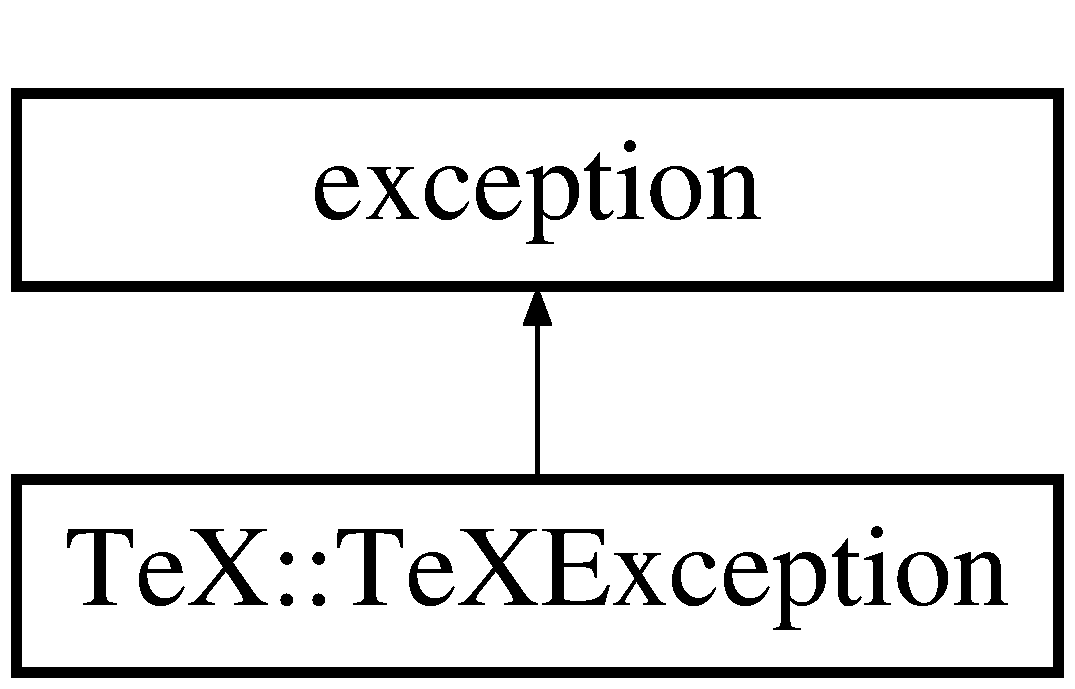
\includegraphics[height=2.000000cm]{class_te_x_1_1_te_x_exception}
\end{center}
\end{figure}
\subsection*{Public Member Functions}
\begin{DoxyCompactItemize}
\item 
{\footnotesize template$<$typename T $>$ }\\\hyperlink{class_te_x_1_1_te_x_exception_a71087ed70be236df40e20fe737a1ba1b}{Te\+X\+Exception} (T \hyperlink{class_te_x_1_1_te_x_exception_a189f589619c4ee5106af390c7a8ac3f5}{what})
\item 
virtual const char $\ast$ \hyperlink{class_te_x_1_1_te_x_exception_a189f589619c4ee5106af390c7a8ac3f5}{what} () const  throw ()
\end{DoxyCompactItemize}


\subsection{Detailed Description}
standard exception for errors happening in this libray 

\subsection{Constructor \& Destructor Documentation}
\mbox{\Hypertarget{class_te_x_1_1_te_x_exception_a71087ed70be236df40e20fe737a1ba1b}\label{class_te_x_1_1_te_x_exception_a71087ed70be236df40e20fe737a1ba1b}} 
\index{Te\+X\+::\+Te\+X\+Exception@{Te\+X\+::\+Te\+X\+Exception}!Te\+X\+Exception@{Te\+X\+Exception}}
\index{Te\+X\+Exception@{Te\+X\+Exception}!Te\+X\+::\+Te\+X\+Exception@{Te\+X\+::\+Te\+X\+Exception}}
\subsubsection{\texorpdfstring{Te\+X\+Exception()}{TeXException()}}
{\footnotesize\ttfamily template$<$typename T $>$ \\
Te\+X\+::\+Te\+X\+Exception\+::\+Te\+X\+Exception (\begin{DoxyParamCaption}\item[{T}]{what }\end{DoxyParamCaption})\hspace{0.3cm}{\ttfamily [inline]}}

sets the message error for the exception considered 

\subsection{Member Function Documentation}
\mbox{\Hypertarget{class_te_x_1_1_te_x_exception_a189f589619c4ee5106af390c7a8ac3f5}\label{class_te_x_1_1_te_x_exception_a189f589619c4ee5106af390c7a8ac3f5}} 
\index{Te\+X\+::\+Te\+X\+Exception@{Te\+X\+::\+Te\+X\+Exception}!what@{what}}
\index{what@{what}!Te\+X\+::\+Te\+X\+Exception@{Te\+X\+::\+Te\+X\+Exception}}
\subsubsection{\texorpdfstring{what()}{what()}}
{\footnotesize\ttfamily virtual const char$\ast$ Te\+X\+::\+Te\+X\+Exception\+::what (\begin{DoxyParamCaption}{ }\end{DoxyParamCaption}) const throw  ) \hspace{0.3cm}{\ttfamily [inline]}, {\ttfamily [virtual]}}

returns the message errror for the exception considered 

The documentation for this class was generated from the following file\+:\begin{DoxyCompactItemize}
\item 
C\+:/\+Users/nicoc\+\_\+000/\+Desktop/\+Grafia/\+Grafia/\+Source/texlib.\+h\end{DoxyCompactItemize}

%--- End generated contents ---

% Index
\backmatter
\newpage
\phantomsection
\clearemptydoublepage
\addcontentsline{toc}{chapter}{Index}
\printindex

\end{document}
